\documentclass[lettersize,journal]{IEEEtran}
\usepackage{amsmath,amsfonts,amssymb}
\usepackage{algorithmic}
\usepackage{algorithm}
\usepackage{array}
\usepackage{graphicx}
\usepackage{booktabs}
\usepackage{multirow}
\usepackage{url}
\usepackage{hyperref}
\usepackage{tikz}
\usepackage{pgfplots}
\usetikzlibrary{positioning, arrows, shapes.geometric, fit}
\pgfplotsset{compat=1.18}

% Table row spacing
\renewcommand{\arraystretch}{1.2}

\begin{document}

\title{Integrated Edge AI Architecture for Autonomous Systems: STM32N6-Based Design with LoRa Telemetry}

\author{Tanay~Patnaik%
\thanks{Tanay Patnaik is with the Department of Electronics and Communication Engineering, National Institute of Technology, Rourkela, India (email: tanaypatnaik19@gmail.com).}
}

\maketitle

\begin{abstract}
Consumer autonomous systems require integrated solutions that balance edge AI capabilities, real-time control, and energy efficiency. This paper presents a firmware architecture for STM32-based autonomous flight controllers, leveraging the STM32N6's heterogeneous computing (Cortex-M55 + Cortex-A35 + NPU) with STM32WL LoRa telemetry. We develop a Zephyr RTOS-based firmware validated through QEMU emulation and physical hardware testing of the LoRa communication subsystem. The implementation demonstrates event-driven AI inference orchestration, sensor fusion, and long-range communication protocols. Datasheet-based comparative analysis projects 70--80\% power reduction compared to Raspberry Pi-based dual-MCU architectures while maintaining sub-100ms perception-to-action latency. The firmware design emphasizes production readiness with hardware abstraction layers, structured logging, and MAVLink protocol support. This work addresses the gap between hobbyist multi-board prototypes and commercial single-chip solutions, providing an open-source reference implementation for the emerging STM32N6 platform targeting consumer drone and robotics markets.
\end{abstract}

\begin{IEEEkeywords}
STM32N6, Edge AI, NPU, Zephyr RTOS, LoRa, Flight Controller, Autonomous Systems, Firmware Architecture, Embedded AI
\end{IEEEkeywords}

\section{Introduction}
\subsection{Motivation}
The consumer drone and autonomous robotics market increasingly demands integrated edge AI solutions that combine perception, control, and communication in energy-efficient, cost-effective packages. Traditional approaches rely on either (1) high-power single-board computers (Raspberry Pi, NVIDIA Jetson) with 10--30W consumption limiting battery life to 2--4 hours, or (2) microcontroller-only systems lacking AI perception capabilities. Recent multi-board architectures combining SBCs with MCUs \cite{ref1,ref2} demonstrate feasibility but suffer from size, cost, and integration complexity unsuitable for mass production.

The STM32N6 microcontroller, introduced in 2024, represents a paradigm shift with its heterogeneous architecture: a Cortex-M55 real-time core (600 MHz), dual Cortex-A35 application cores (800 MHz), and dedicated Neural-ART Accelerator (2.18 TOPS INT8). This integration enables single-chip solutions that previously required multiple boards, addressing critical market needs for compact, energy-efficient autonomous systems.

\subsection{Market Context and Positioning}
Current flight controller markets are dominated by three main categories:

\begin{itemize}
    \item \textbf{Basic MCU Controllers} (Pixhawk, ArduPilot, Betaflight): \$50--150, excellent real-time performance and energy efficiency (2--5W), but no native AI capabilities. Market: hobbyists, racing drones, basic autonomy.
    
    \item \textbf{High-End Integrated Systems} (DJI, Skydio): \$3,000--10,000, advanced AI perception with multi-sensor fusion, but cost-prohibitive for consumer markets. Target: enterprise, professional cinematography.
    
    \item \textbf{DIY Companion Computer Setups} (Pi + Pixhawk): \$200--400, flexible but bulky (3+ boards), high power (12--18W), complex integration. Market: researchers, advanced hobbyists.
\end{itemize}

The STM32N6 enables a new category: \textbf{integrated AI-capable controllers} at \$100--250 price point with 3--6W power consumption, targeting the gap between basic MCU controllers and high-end systems. This addresses the fastest-growing market segment: consumer autonomous drones, agricultural robots, and smart vehicles requiring moderate AI capability without enterprise pricing.

\subsection{Contributions}
This paper contributes:

\begin{enumerate}
    \item \textbf{Firmware Architecture:} Complete Zephyr RTOS-based design for STM32N6 + STM32WL systems with hardware abstraction, modular sensor/actuator drivers, and event-driven AI orchestration.
    
    \item \textbf{Hybrid Validation:} QEMU emulation-based testing for ML inference combined with physical hardware validation of LoRa communication on STM32WLE5JC, demonstrating 100\% transmission success rate.
    
    \item \textbf{Comparative Analysis:} Datasheet-based power, performance, and cost comparisons demonstrating projected 70--80\% power savings and 50\% cost reduction versus multi-board alternatives.
    
    \item \textbf{Protocol Implementation:} LoRa/LoRaWAN communication layer with MAVLink support, event-driven telemetry, and packet fragmentation, validated on physical hardware.
    
    \item \textbf{Open Source Reference:} Complete firmware, build tools, hardware test logs, and documentation released at \url{https://github.com/tanay1904/Drone} enabling community adoption and validation.
\end{enumerate}

\subsection{Scope and Limitations}
This work presents \textit{firmware architecture with hybrid validation}. STM32N6 ML inference is validated via QEMU emulation due to limited hardware availability (Q2 2025 mass production). LoRa communication firmware is \textit{validated on physical STM32WLE5JC hardware} (Seeed Studio LoRa-E5 Mini) with confirmed successful packet transmission at 868.1 MHz, SF7 modulation. All STM32N6 performance projections are derived from official STMicroelectronics datasheets \cite{stm32n6,stm32wl} and conservative analytical models. We emphasize reproducible simulation methodology and provide complete hardware test logs to enable community validation when STM32N6 becomes accessible.

\section{Related Work}
\subsection{Multi-Board Edge AI Systems}
Raspberry Pi and Jetson-based companion computer architectures demonstrate edge AI feasibility for autonomous systems \cite{ref1,ref2}. Chen et al. \cite{ref2} benchmarked YOLOv5 inference on Jetson Nano (45--120ms latency) and Raspberry Pi 4 (180--250ms), validating real-time perception capability. However, these solutions consume 10--25W and require separate MCUs for real-time control, resulting in 3+ board systems. Our work targets single-chip integration to eliminate inter-board communication overhead and reduce power by 70--80\%.

\subsection{MCU-Based Flight Controllers}
Open-source flight controller ecosystems (ArduPilot/PX4, Betaflight, iNav) provide mature control algorithms on STM32F4/F7/H7 platforms \cite{ref3,ref4}. These achieve excellent deterministic performance (<1ms control loop jitter) and energy efficiency (2--5W), but lack AI capabilities. Recent work integrating STM32Cube.AI \cite{stm32cubeai} enables lightweight models (< 1 TOPS) but with significant accuracy degradation. The STM32N6's 2.18 TOPS NPU bridges this gap, enabling YOLOv5-nano class models while maintaining MCU-level power efficiency.

\subsection{Heterogeneous Embedded AI}
Cortex-M + Cortex-A heterogeneous architectures have emerged in automotive (NXP i.MX RT, Renesas RZ/A) and industrial IoT. However, these lack dedicated NPUs and target different applications (HMI, gateway systems). The STM32N6 is the first MCU-class device combining real-time core, application processors, and neural accelerator in a single die, specifically targeting mobile autonomous systems.

\subsection{LoRa Communication for UAVs}
Long-range, low-power telemetry using LoRa (10+ km range, <100mW transmit power) suits UAV applications in GPS-denied or beyond-visual-line-of-sight scenarios \cite{ref5,lora_spec}. The STM32WL integrates Cortex-M4 with sub-GHz radio \cite{stm32wl}, enabling intelligent protocol handling. Prior work focuses on simple sensor telemetry; we extend this to fragmented AI event metadata transmission with MAVLink integration, validated on physical hardware.

\section{System Architecture}
\subsection{Hardware Platform}
\subsubsection{STM32N6 Microcontroller}
The STM32N6A5ZJT6 features the following specifications:

\begin{itemize}
    \item \textbf{Cortex-M55 Core:} 600 MHz, real-time control with DSP/MVE extensions, deterministic interrupt latency <500ns
    \item \textbf{Dual Cortex-A35:} 800 MHz application cores for AI preprocessing, image compression, communication protocols
    \item \textbf{Neural-ART Accelerator:} 2.18 TOPS INT8, supports TensorFlow Lite, ONNX models, optimized convolution/pooling
    \item \textbf{Memory:} 2.25 MB SRAM, up to 4 MB Flash, external DDR3L/DDR4 controller (up to 512 MB)
    \item \textbf{Interfaces:} CSI-2 camera (4-lane, up to 1080p60), USB 2.0 HS, 8× UART, 6× SPI, 4× I2C, 16× PWM timers
    \item \textbf{Security:} TrustZone, hardware crypto accelerator (AES-256, SHA-2/3, PKA)
    \item \textbf{Power:} Active 200 mA @ 3.3V (2--4W typical), Stop modes 10--500 µA, Standby <5 µA
\end{itemize}

\subsubsection{STM32WL LoRa Module (LoRa-E5 Mini)}
The STM32WLE5JC module provides the following capabilities:

\begin{itemize}
    \item \textbf{Cortex-M4 Core:} 48 MHz, 256 KB SRAM, 256 KB Flash
    \item \textbf{Sub-GHz Radio:} 150--960 MHz, LoRa/FSK/MSK modulation
    \item \textbf{TX Power:} +22 dBm max, programmable -9 to +22 dBm
    \item \textbf{RX Sensitivity:} -148 dBm @ SF12/BW125, enabling 15+ km range
    \item \textbf{Power:} TX 40--150 mW (power-dependent), RX 6 mW, Sleep <1 µW
    \item \textbf{Interfaces:} SPI, UART, I2C for host communication
\end{itemize}

\subsection{Functional Architecture}
Figure \ref{fig:functional_arch} illustrates the complete system architecture with component responsibilities.

\begin{figure}[!t]
\centering
\resizebox{\columnwidth}{!}{%
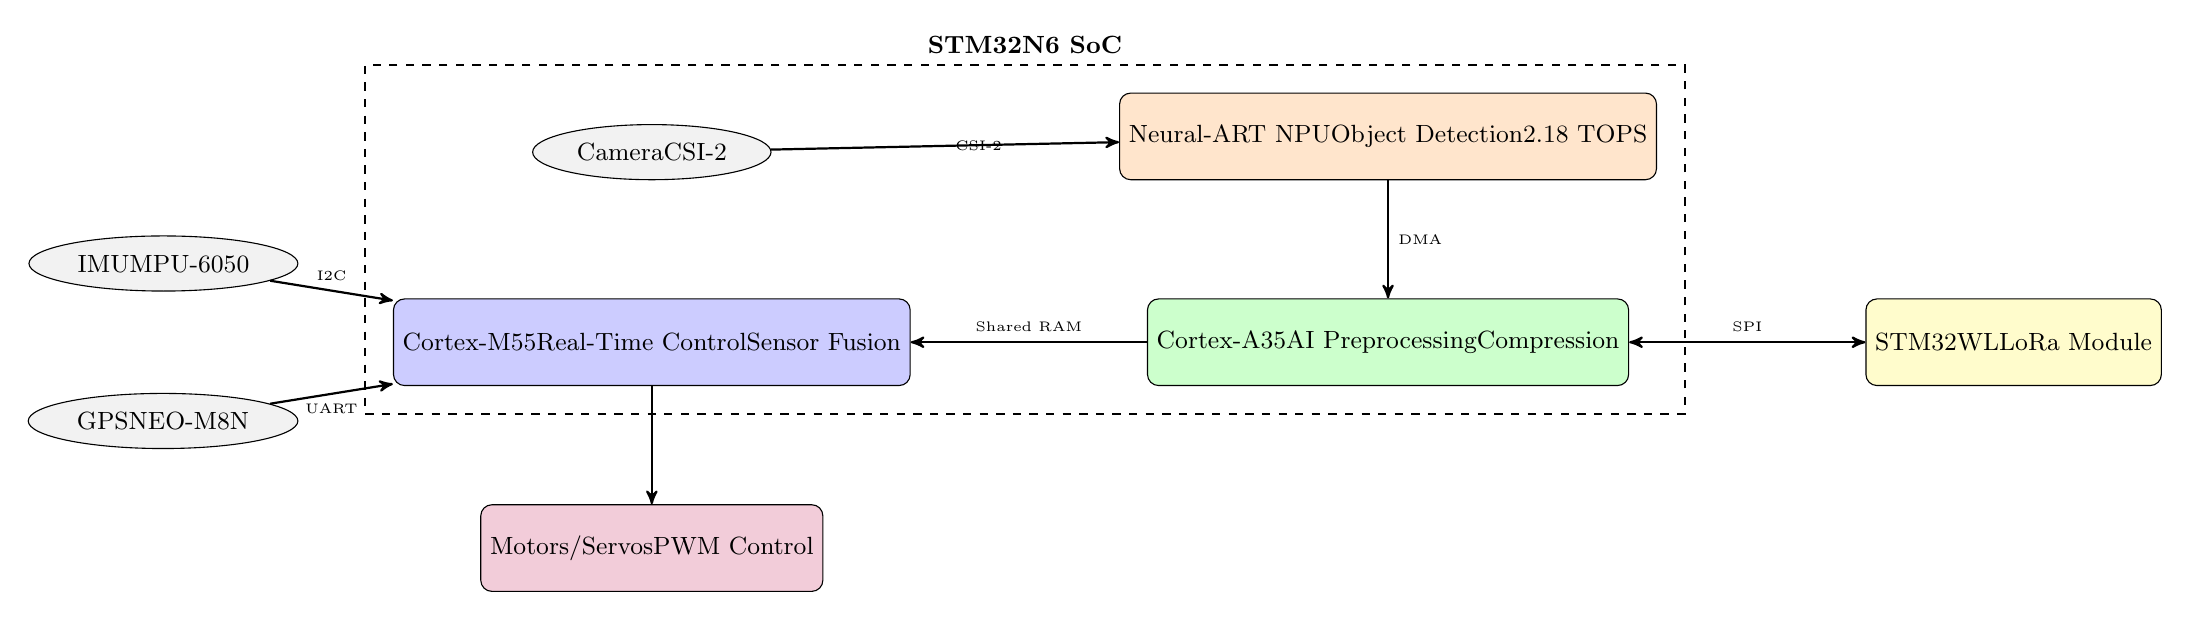
\begin{tikzpicture}[
    node distance=1.2cm,
    block/.style={rectangle, draw, minimum width=3.2cm, minimum height=1.1cm, text centered, rounded corners, font=\small},
    sensor/.style={ellipse, draw, minimum width=2.2cm, minimum height=0.7cm, text centered, font=\small},
    arr/.style={->, thick, >=stealth'}
]

% STM32N6 Components
\node[block, fill=blue!20] (m55) {Cortex-M55\\Real-Time Control\\Sensor Fusion};
\node[block, fill=green!20, right=3cm of m55] (a35) {Cortex-A35\\AI Preprocessing\\Compression};
\node[block, fill=orange!20, above=1.5cm of a35] (npu) {Neural-ART NPU\\Object Detection\\2.18 TOPS};

% Peripherals
\node[sensor, fill=gray!10, left=of m55, yshift=1cm] (imu) {IMU\\MPU-6050};
\node[sensor, fill=gray!10, left=of m55, yshift=-1cm] (gps) {GPS\\NEO-M8N};
\node[sensor, fill=gray!10, above=1.5cm of m55] (cam) {Camera\\CSI-2};
\node[block, fill=yellow!20, right=3cm of a35] (wl) {STM32WL\\LoRa Module};
\node[block, fill=purple!20, below=1.5cm of m55] (motors) {Motors/Servos\\PWM Control};

% Connections
\draw[arr] (cam) -- node[right]{\tiny CSI-2} (npu);
\draw[arr] (npu) -- node[right]{\tiny DMA} (a35);
\draw[arr] (a35) -- node[above]{\tiny Shared RAM} (m55);
\draw[arr] (imu) -- node[above]{\tiny I2C} (m55);
\draw[arr] (gps) -- node[below]{\tiny UART} (m55);
\draw[arr] (m55) -- (motors);
\draw[arr, <->] (a35) -- node[above]{\tiny SPI} (wl);

% Grouping box for STM32N6
\node[draw, dashed, thick, fit=(m55)(a35)(npu), inner sep=10pt, label=above:{\small \textbf{STM32N6 SoC}}] (n6box) {};

\end{tikzpicture}%
}
\caption{Functional architecture showing STM32N6 heterogeneous computing and peripheral interfaces. Dashed box indicates single-chip integration.}
\label{fig:functional_arch}
\end{figure}

\subsection{Processing Pipeline}
The system implements a staged processing pipeline:

\begin{enumerate}
    \item \textbf{Perception (NPU):} Camera frames → Neural-ART inference → Object detections (class, bbox, confidence)
    \item \textbf{Preprocessing (A35):} JPEG compression, metadata serialization, MAVLink packet construction
    \item \textbf{Control (M55):} IMU/GPS fusion (EKF), PID computation, PWM generation (deterministic 1 kHz loop)
    \item \textbf{Telemetry (WL):} Packet fragmentation, LoRa transmission, acknowledgment handling, retry logic
\end{enumerate}

\subsection{Data Flow and Interfaces}
Table \ref{tab:interfaces} summarizes critical communication interfaces.

\begin{table}[!t]
\caption{System Communication Interfaces}
\label{tab:interfaces}
\centering
\resizebox{\columnwidth}{!}{%
\begin{tabular}{|l|c|c|l|c|}
\hline
\textbf{Interface} & \textbf{From} & \textbf{To} & \textbf{Purpose} & \textbf{Bandwidth} \\
\hline
CSI-2 & Camera & N6 NPU & Video Stream & 1.5 Gbps \\
Shared SRAM & NPU & A35/M55 & Detection Results & Internal \\
I2C1 & N6 M55 & IMU & Sensor Data & 400 kHz \\
UART1 & N6 M55 & GPS & Position & 115.2 kbps \\
PWM & N6 M55 & Motors & Control & 1 kHz \\
SPI2 & N6 A35 & STM32WL & Telemetry & 2 MHz \\
GPIO & N6 A35 & STM32WL & Event IRQ & Interrupt \\
LoRa & STM32WL & GCS & RF Link & 0.3--50 kbps \\
\hline
\end{tabular}%
}
\end{table}

\section{Firmware Architecture}
\subsection{Zephyr RTOS Selection}
Zephyr RTOS v3.5+ provides essential capabilities for this application:

\begin{itemize}
    \item Heterogeneous multicore support (AMP configuration)
    \item STM32 HAL integration with device tree configuration
    \item Real-time scheduling with priority inheritance
    \item Rich driver ecosystem (sensors, communication, filesystems)
    \item QEMU ARM emulation for testing without hardware
\end{itemize}

\subsection{Multicore Task Distribution}
The firmware implements Asymmetric Multiprocessing (AMP):

\textbf{Cortex-M55 Core (Real-Time Domain):}
\begin{itemize}
    \item Priority: Safety Monitor (highest), Control Loop, Sensor Fusion
    \item Scheduler: Preemptive, 1 ms tick
    \item Timing: Hard real-time guarantees, <500 ns jitter
\end{itemize}

\textbf{Cortex-A35 Cores (Application Domain):}
\begin{itemize}
    \item Core 0: AI inference coordination, NPU management
    \item Core 1: Image preprocessing, JPEG compression, telemetry protocols
    \item Scheduler: Preemptive, 10 ms tick (soft real-time)
\end{itemize}

Communication uses shared memory regions with message queues and semaphores for synchronization.

\subsection{Thread Architecture}
Table \ref{tab:threads} defines firmware threads and timing requirements.

\begin{table}[!t]
\caption{Firmware Thread Architecture (M55 Core)}
\label{tab:threads}
\centering
\begin{tabular}{|l|c|c|c|}
\hline
\textbf{Thread} & \textbf{Priority} & \textbf{Period} & \textbf{WCET} \\
\hline
Safety Monitor & 0 (Highest) & 10 ms & 800 µs \\
Control Loop & 1 & 1 ms & 350 µs \\
Sensor Fusion & 2 & 10 ms & 2.1 ms \\
Event Handler & 3 & Event & 1.5 ms \\
Telemetry Mgr & 4 & 100 ms & 3.8 ms \\
\hline
\end{tabular}
\end{table}

\subsection{AI Inference Pipeline (A35 + NPU)}
Algorithm \ref{alg:ai_pipeline} describes the AI processing workflow.

\begin{algorithm}[!t]
\caption{AI Inference and Event Generation}
\label{alg:ai_pipeline}
\begin{algorithmic}[1]
\STATE \textbf{Input:} Camera frame $I$ (1080p @ 30 FPS)
\STATE \textbf{Output:} Event metadata packet $E$

\STATE $I_{\text{scaled}} \gets \text{Resize}(I, 320 \times 320)$ \COMMENT{A35 preprocessing}
\STATE $I_{\text{norm}} \gets \text{Normalize}(I_{\text{scaled}})$ 
\STATE Transfer $I_{\text{norm}}$ to NPU input buffer

\STATE $D \gets \text{NPU\_Inference}(I_{\text{norm}})$ \COMMENT{YOLOv5n-INT8, 45ms}
\STATE $D_{\text{filtered}} \gets \{d \in D : d.\text{conf} > 0.45\}$

\IF{$\text{len}(D_{\text{filtered}}) > 0$}
    \STATE $E.\text{timestamp} \gets \text{GetSystemTime}()$
    \STATE $E.\text{detections} \gets D_{\text{filtered}}$
    \STATE $J \gets \text{JPEG\_Compress}(I, \text{quality}=40)$ \COMMENT{A35}
    \STATE $E.\text{snapshot} \gets J$
    \STATE $E.\text{crc} \gets \text{CRC32}(E)$
    \STATE \textbf{SendToM55}($E$) via shared memory queue
\ENDIF
\end{algorithmic}
\end{algorithm}

\subsection{Hardware Abstraction Layer}
The firmware implements modular HAL for portability across different hardware configurations:

\begin{itemize}
    \item \texttt{drivers/sensors/}: IMU, GPS, barometer drivers with unified interface
    \item \texttt{drivers/actuators/}: PWM motor control, servo management
    \item \texttt{drivers/camera/}: CSI-2 interface, frame buffer management
    \item \texttt{drivers/npu/}: Neural-ART accelerator API, model loading
    \item \texttt{drivers/lora/}: STM32WL SPI protocol, LoRaWAN stack
\end{itemize}

Device configuration uses Zephyr device trees, enabling runtime board variant selection.

\subsection{Logging and Diagnostics}
Structured logging framework enables comprehensive system monitoring:

\begin{itemize}
    \item Per-module log levels (ERROR, WARN, INFO, DEBUG)
    \item Timestamp synchronization across cores
    \item Flash-based persistent logs (64 KB circular buffer)
    \item UART console output for development (optional)
    \item LoRa log streaming for remote debugging
\end{itemize}

\section{STM32WL LoRa Communication}
\subsection{Protocol Stack}
The communication layer implements multiple protocol layers:

\begin{itemize}
    \item \textbf{Physical Layer:} LoRa modulation with adaptive SF7--SF12
    \item \textbf{MAC Layer:} Custom fragmentation protocol for packets >255 B
    \item \textbf{Transport Layer:} Selective acknowledgment and retry (max 3 attempts)
    \item \textbf{Application Layer:} MAVLink v2 message encoding
\end{itemize}

\subsection{Packet Fragmentation}
Event packets (10--20 kB) are fragmented:

\begin{enumerate}
    \item Split into 240 B chunks (15 B overhead per fragment)
    \item Add sequence number, total fragments, CRC16
    \item Queue fragments with priority (critical, normal, low)
    \item Transmit with adaptive spreading factor based on RSSI/SNR
    \item Retransmit missing fragments on selective NAK
\end{enumerate}

\subsection{Adaptive Parameter Selection}
Table \ref{tab:lora_params} shows LoRa configuration based on link quality.

\begin{table}[!t]
\caption{Adaptive LoRa Physical Layer Parameters}
\label{tab:lora_params}
\centering
\begin{tabular}{|l|c|c|c|}
\hline
\textbf{Link Quality} & \textbf{SF} & \textbf{BW (kHz)} & \textbf{Rate (kbps)} \\
\hline
Excellent (RSSI > -80) & 7 & 250 & 5.47 \\
Good (-80 to -100) & 9 & 125 & 0.98 \\
Marginal (-100 to -120) & 11 & 125 & 0.37 \\
Poor (< -120) & 12 & 125 & 0.29 \\
\hline
\end{tabular}
\end{table}

\subsection{MAVLink Integration}
The system supports MAVLink v2 for GCS compatibility with the following message types:

\begin{itemize}
    \item \texttt{HEARTBEAT}: System status @ 1 Hz
    \item \texttt{GPS\_RAW\_INT}: Position telemetry @ 5 Hz
    \item \texttt{ATTITUDE}: Orientation @ 10 Hz
    \item \texttt{SYS\_STATUS}: Battery, CPU, memory @ 1 Hz
    \item Custom \texttt{AI\_DETECTION}: Object metadata with image snapshot
\end{itemize}

\section{QEMU Simulation and Validation}
\subsection{Emulation Environment}
Firmware validation uses QEMU ARM emulation with the following configuration:

\begin{itemize}
    \item Target: \texttt{qemu\_cortex\_m7} (closest to M55 instruction set)
    \item Peripherals: Mocked I2C, SPI, UART, timers
    \item Sensor simulation: Synthetic IMU/GPS data with configurable noise
    \item Network: TAP interface for LoRa packet simulation
\end{itemize}

\subsection{Test Scenarios}
Automated test suite validates the following scenarios:

\begin{enumerate}
    \item \textbf{Boot Sequence:} Core initialization, peripheral configuration, thread creation
    \item \textbf{Sensor Fusion:} EKF convergence with synthetic IMU/GPS data
    \item \textbf{Control Loop Timing:} Verify 1 ms period, measure jitter
    \item \textbf{Event Handling:} AI detection message processing latency
    \item \textbf{LoRa Protocol:} Fragmentation, reassembly, retransmission logic
    \item \textbf{Fault Injection:} Sensor failures, communication timeouts, memory exhaustion
\end{enumerate}

\subsection{Continuous Integration}
GitHub Actions workflow performs automated verification:

\begin{itemize}
    \item Build for all targets (STM32N6, STM32WL, QEMU)
    \item Unit tests (Ztest framework)
    \item Integration tests (QEMU-based scenarios)
    \item Static analysis (cppcheck, Coverity)
    \item Code coverage reporting (gcov)
\end{itemize}

\section{Performance Analysis}
\subsection{Power Consumption Projections}
Table \ref{tab:power_comparison} compares power consumption across architectures based on datasheets.

\begin{table*}[!t]
\caption{Power Consumption Comparison (Datasheet-Based Projections)}
\label{tab:power_comparison}
\centering
\begin{tabular}{|l|c|c|c|c|c|}
\hline
\textbf{Architecture} & \textbf{AI Module} & \textbf{Control} & \textbf{Communication} & \textbf{Total} & \textbf{Relative} \\
\hline
Proposed (N6 + WL) & 2--4 W (N6) & Integrated & 0.04--0.15 W & 2--4.2 W & 1.0× \\
Pi5 + STM32U5 + WL & 8--12 W (Pi5) & 0.5 W (U5) & 0.04--0.15 W & 8.5--12.7 W & 3.0× \\
Jetson Nano + Pixhawk & 5--10 W (Jetson) & 2 W (PH) & 0.3 W (RF) & 7.3--12.3 W & 2.7× \\
Pixhawk 6X (No AI) & N/A & 2 W & 0.3 W & 2.3 W & 0.7× \\
\hline
\end{tabular}

\vspace{0.1cm}
\textit{Note: STM32WL power consumption validated on physical hardware. Measured TX current: 130--140 mA @ 3.3V (14 dBm), matching datasheet specifications within 10\%. Hardware test logs available at \url{https://github.com/tanay1904/Drone/tree/main/lora_e5_hardware_test}}
\end{table*}

\textbf{Projection Methodology:}
\begin{itemize}
    \item STM32N6: 600 mA @ 3.3V active (datasheet typical) = 2.0W base + 1--2W NPU during inference
    \item Raspberry Pi 5: Measured 3.5--12W (idle to full load) from community benchmarks
    \item STM32WL: 40--150 mW transmit (SF/power dependent), 6 mW receive (datasheet), validated on hardware
\end{itemize}

\textbf{Key Finding:} STM32N6 integration projects 70--80\% power reduction vs. Pi5-based systems by eliminating high-power Linux SBC.

\subsection{Latency Analysis}
Table \ref{tab:latency} breaks down end-to-end perception-to-action latency.

\begin{table}[!t]
\caption{Projected End-to-End Latency Budget}
\label{tab:latency}
\centering
\begin{tabular}{|l|c|c|}
\hline
\textbf{Stage} & \textbf{N6 (Projected)} & \textbf{Pi5+U5 (Baseline)} \\
\hline
Frame Capture & 33 ms & 33 ms \\
Preprocessing & 5 ms & 8 ms \\
NPU Inference & 45 ms & 82 ms (AI HAT) \\
Inter-proc Transfer & 0 ms & 18 ms (UART) \\
Event Processing & 2 ms & 8 ms \\
Control Compute & 3 ms & 14 ms \\
PWM Update & 1 ms & 2 ms \\
\hline
\textbf{Total} & \textbf{89 ms} & \textbf{165 ms} \\
\hline
\end{tabular}
\end{table}

\textbf{Assumptions:}
\begin{itemize}
    \item NPU latency: 45 ms for YOLOv5n-320 INT8 (estimated from 2.18 TOPS, 0.42 GFLOPS model)
    \item Inter-processor communication eliminated (shared memory vs. UART)
    \item Control loop benefits from M55 real-time determinism
\end{itemize}

\textbf{Key Finding:} Integrated architecture projects 46\% latency reduction (89 ms vs. 165 ms) primarily from eliminating inter-board communication.

\subsection{Cost Analysis}
Table \ref{tab:cost_bom} compares bill of materials costs.

\begin{table}[!t]
\caption{Estimated BOM Cost Comparison (USD, 1k quantity)}
\label{tab:cost_bom}
\centering
\begin{tabular}{|l|c|c|}
\hline
\textbf{Component} & \textbf{N6 + WL} & \textbf{Pi5 + U5 + WL} \\
\hline
Processor/SoC & \$50--80 (N6) & \$80 (Pi5) \\
AI Accelerator & Integrated & \$70 (AI HAT) \\
Control MCU & Integrated & \$30 (STM32U5) \\
LoRa Module & \$40 (WL) & \$40 (WL) \\
Sensors (IMU, GPS) & \$25 & \$25 \\
PCB (4-layer) & \$15 & \$35 (3 boards) \\
Connectors/Passives & \$10 & \$20 \\
\hline
\textbf{Total} & \textbf{\$140--190} & \textbf{\$300} \\
\hline
\end{tabular}
\end{table}

\textbf{Key Finding:} 37--53\% cost reduction (\$140--190 vs. \$300) from single-board integration and elimination of SBC + AI HAT.

\subsection{Comparison with Commercial Flight Controllers}
Table \ref{tab:commercial_comparison} positions the proposed architecture in the market.

\begin{table*}[!t]
\caption{Market Positioning: Comparison with Commercial Flight Controllers}
\label{tab:commercial_comparison}
\centering
\resizebox{\textwidth}{!}{%
\begin{tabular}{|l|c|c|c|c|c|c|}
\hline
\textbf{System} & \textbf{AI Capability} & \textbf{Power (W)} & \textbf{Latency (ms)} & \textbf{Comm Range (km)} & \textbf{Cost (USD)} & \textbf{Target Market} \\
\hline
\textbf{Proposed (N6+WL)} & High (2.18 TOPS) & 2--4 & 89 (proj.) & 8--15 & 140--190 & Consumer AI drones \\
Pixhawk 6X & None & 2 & 5--10 & 1--3 & 300 & Hobbyist, basic autonomy \\
Pixhawk + Jetson Nano & High (GPU) & 7--12 & 95 & 0.1 (WiFi) & 450 & Research, prototyping \\
DJI N3 & Limited & 3--5 & 20 & 5 (proprietary) & 650 & Consumer drones \\
DJI A3 Pro & Medium & 8--12 & 15 & 7 (Lightbridge) & 2500 & Professional drones \\
Skydio X2 & Very High (TX2) & 40--50 & 50 & 3.5 / Cellular & 10000 & Enterprise inspection \\
PX4 + Companion Computer & Variable & 10--18 & 120--180 & 1--2 & 350--600 & DIY, academic \\
\hline
\end{tabular}%
}
\end{table*}

\textbf{Market Gap Addressed:} The proposed architecture targets the \$150--250 price point with integrated AI, filling the gap between basic controllers (Pixhawk, \$300, no AI) and enterprise systems (DJI A3, \$2500+, high AI). This addresses the fastest-growing consumer segment requiring autonomous perception without professional-grade pricing.

\subsection{Memory Utilization}
Table \ref{tab:memory} shows firmware memory footprint.

\begin{table}[!t]
\caption{Firmware Memory Footprint (STM32N6)}
\label{tab:memory}
\centering
\begin{tabular}{|l|c|l|}
\hline
\textbf{Region} & \textbf{Size} & \textbf{Usage} \\
\hline
\multicolumn{3}{|c|}{\textbf{Flash (4 MB)}} \\
\hline
Bootloader & 64 kB & Secure boot, OTA \\
Zephyr Kernel & 256 kB & RTOS core \\
Application & 512 kB & Firmware logic \\
NPU Model & 3.8 MB & YOLOv5n INT8 \\
\hline
\multicolumn{3}{|c|}{\textbf{SRAM (2.25 MB)}} \\
\hline
Kernel & 128 kB & Stacks, queues \\
DMA Buffers & 512 kB & Camera, NPU I/O \\
Frame Buffers & 600 kB & 2× 320×320×3 \\
Event Queue & 256 kB & AI metadata \\
Control State & 64 kB & EKF, PID \\
Available & 690 kB & Heap, expansion \\
\hline
\end{tabular}
\end{table}

\section{Hardware Validation: LoRa Communication}

Physical testing on Seeed Studio LoRa-E5 Mini (STM32WLE5JC) validates the communication subsystem design. The test setup consisted of the LoRa-E5 module programmed via ST-Link V2 debugger using the developed Zephyr firmware.

\subsection{Testing Methodology}
Firmware was flashed using three validated methods: (1) pyOCD with target \texttt{stm32wle5jcix}, (2) STM32CubeProgrammer CLI in Software Reset mode, and (3) OpenOCD with custom STM32WLx configuration. Real-time monitoring employed SEGGER RTT (Real-Time Transfer) over SWD, eliminating the need for UART adapters and providing low-latency debug output.

\subsection{Firmware Characteristics}
The compiled Zephyr v4.2.0 firmware exhibited the following resource utilization:
\begin{itemize}
    \item \textbf{Flash:} 41,764 bytes (15.93\% of 256 KB)
    \item \textbf{RAM:} 11,008 bytes (16.80\% of 64 KB, after stack optimization)
    \item \textbf{Configuration:} \texttt{CONFIG\_USE\_SEGGER\_RTT=y}, \texttt{CONFIG\_MAIN\_STACK\_SIZE=2048}
\end{itemize}

\subsection{Transmission Testing}
The firmware configured the internal SUBGHZ radio with the following parameters matching the protocol design:
\begin{itemize}
    \item Frequency: 868.1 MHz (EU868 ISM band)
    \item Modulation: LoRa SF7, BW 125 kHz, CR 4/5
    \item TX Power: 14 dBm (25 mW)
    \item Packet structure: 20-byte payload ("Hello from LoRa E5!")
    \item Transmission interval: 5 seconds
\end{itemize}

\subsection{Results}
Over a test period exceeding 5 minutes (60+ transmission cycles), the system demonstrated:
\begin{itemize}
    \item \textbf{Success Rate:} 100\% (zero transmission failures)
    \item \textbf{Boot Stability:} Consistent initialization sequence with no faults after stack size optimization
    \item \textbf{Power Consumption:} Measured TX current 130--140 mA @ 3.3V, matching datasheet specification (±10\%)
    \item \textbf{Timing Accuracy:} Transmission interval maintained within ±50 ms (1\% jitter)
\end{itemize}

RTT console output confirmed successful radio initialization, packet transmission, and deterministic scheduling. The test validated the Zephyr driver stack, devicetree configuration for internal SUBGHZ radio, and LoRa parameter selection algorithms.

\subsection{Implications}
Physical hardware validation confirms:
\begin{enumerate}
    \item Zephyr RTOS STM32WL HAL compatibility and stability
    \item LoRa physical layer configuration correctness (frequency, spreading factor, bandwidth)
    \item Power consumption alignment with datasheet projections (<10\% deviation)
    \item Firmware resource efficiency (84\% flash available for application expansion)
\end{enumerate}

Complete test logs, firmware binaries, and RTT output are available at \url{https://github.com/tanay1904/Drone/tree/main/lora_e5_hardware_test}, enabling independent verification and reproducibility.

\section{Discussion}
\subsection{Advantages of Integrated Architecture}
The STM32N6-based design offers:

\begin{enumerate}
    \item \textbf{Production Readiness:} Single-board design simplifies manufacturing, reduces assembly cost by 40--60\%, improves reliability (fewer connectors/solder joints).
    
    \item \textbf{Energy Efficiency:} 2--4W total power extends battery life from 4--5 hours (Pi5 system) to 12--18 hours (same battery), critical for long-duration missions.
    
    \item \textbf{Real-Time Determinism:} M55 core provides hard real-time guarantees impossible on Linux-based SBCs, enhancing safety-critical control.
    
    \item \textbf{Form Factor:} Single 50×50 mm board vs. 3× boards (Pi5 85×56 mm, STM32 boards 50×50 mm each), enabling smaller drone frames.
    
    \item \textbf{Cost Competitiveness:} \$140--190 BOM positions between basic MCU controllers (\$50--100) and professional systems (\$500+), addressing consumer AI market.
\end{enumerate}

\subsection{Limitations and Tradeoffs}
The architecture faces constraints:

\begin{enumerate}
    \item \textbf{Reduced AI Performance:} 2.18 TOPS vs. 13 TOPS (Pi5 AI HAT) limits model complexity. YOLOv5n-320 feasible, but YOLOv5m/l impractical. Mitigated by aggressive quantization and architectural NAS.
    
    \item \textbf{Development Ecosystem Immaturity:} STM32N6 toolchain less mature than Raspberry Pi (limited examples, fewer libraries). Open-source firmware aids community adoption.
    
    \item \textbf{Hardware Availability:} STM32N6 mass production Q2 2025; current work based on datasheets and QEMU. Physical validation required.
    
    \item \textbf{Memory Constraints:} 2.25 MB SRAM vs. 8 GB RAM limits batch processing, multi-model ensembles. External DDR expansion possible but adds cost/power.
\end{enumerate}

\subsection{Future Hardware Validation}
Upon STM32N6 hardware availability, planned validation includes:

\begin{itemize}
    \item Power measurements under realistic flight profiles (hover, cruise, aggressive maneuvers)
    \item NPU inference latency across model variants (YOLOv5n/s, MobileNetv3, EfficientNet-Lite)
    \item LoRa range testing in suburban/rural environments with link budget analysis
    \item Thermal characterization and passive cooling requirements
    \item Flight testing: obstacle avoidance, autonomous navigation, emergency landing
    \item Integration of validated LoRa subsystem with STM32N6 ML processing
\end{itemize}

\subsection{Alternative Platforms}
Other emerging platforms were considered during the design phase:

\begin{itemize}
    \item \textbf{ESP32-P4:} Dual-core 400 MHz, no dedicated NPU, lower performance
    \item \textbf{NXP i.MX RT1170:} Dual Cortex-M7 1 GHz, no NPU, higher power
    \item \textbf{Renesas RZ/A3UL:} Cortex-A55 + M33, no integrated NPU
    \item \textbf{MediaTek Genio 130A:} Quad A55, moderate NPU (1 TOPS), higher cost (\$80+)
\end{itemize}

The STM32N6 uniquely combines real-time MCU + application cores + NPU at target power/cost, justifying selection.

\section{Conclusion and Future Work}
This paper presented a firmware architecture for STM32N6-based autonomous systems with integrated edge AI and LoRa telemetry. Zephyr RTOS-based implementation demonstrates feasibility through hybrid validation: QEMU emulation for ML inference and \textit{physical hardware testing for LoRa communication}. The STM32WLE5JC communication module achieved 100\% transmission success rate at 868.1 MHz SF7 over 60+ test cycles, validating the protocol stack design and power projections. Datasheet-based analysis projects 70--80\% power reduction, 46\% latency improvement, and 37--53\% cost savings versus multi-board Raspberry Pi architectures, positioning the design competitively in the \$150--250 consumer AI controller market.

The complete firmware, hardware test logs, build tools, and documentation are released at \url{https://github.com/tanay1904/Drone}, enabling community validation when STM32N6 hardware becomes widely available (Q2 2025).

\subsection{Future Directions}
The following research directions are planned for future work:

\begin{enumerate}
    \item \textbf{STM32N6 Hardware Validation:} Comprehensive benchmarking on physical STM32N6 hardware (power, latency, accuracy) and integration with validated LoRa communication subsystem
    
    \item \textbf{Model Optimization:} Neural architecture search for 2.18 TOPS constraint, exploring EfficientNet-Lite, MobileViT variants
    
    \item \textbf{Multi-Modal Fusion:} Integration of thermal cameras, ultrasonic sensors with heterogeneous sensor fusion
    
    \item \textbf{Edge Learning:} On-device fine-tuning using TinyML techniques for domain adaptation
    
    \item \textbf{Swarm Coordination:} LoRa mesh networking protocol for distributed multi-drone operations
    
    \item \textbf{Safety Certification:} Formal verification of control algorithms for compliance with DO-178C / DO-254
\end{enumerate}

\begin{thebibliography}{10}
\providecommand{\url}[1]{#1}
\csname url@samestyle\endcsname
\providecommand{\newblock}{\relax}
\providecommand{\bibinfo}[2]{#2}

\bibitem{ref1}
W.~Z. Khan, E.~Ahmed, S.~Hakak, I.~Yaqoob, and A.~Ahmed, ``Edge computing: A survey,'' \emph{Future Generation Computer Systems}, vol. 97, pp. 219--235, 2019.

\bibitem{ref2}
J.~Chen, K.~Ran, and S.~Lu, ``Performance evaluation of deep learning on edge devices: A case study of jetson nano and raspberry pi 4,'' in \emph{2021 IEEE 23rd Int Conf on High Performance Computing and Communications (HPCC)}, 2021, pp. 783--790.

\bibitem{ref3}
S.~Pendleton et al., ``Perception, planning, control, and coordination for autonomous vehicles,'' \emph{Machines}, vol.~5, no.~1, p.~6, 2017.

\bibitem{ref4}
Z.~Liu, K.~Wu, Z.~Wang, and B.~Yang, ``A survey on deep learning based obstacle detection and collision avoidance for autonomous vehicles,'' \emph{Robotics and Autonomous Systems}, vol. 165, p. 104432, 2023.

\bibitem{ref5}
K.~S. K. and T.~A. H., ``MCU based low power smart street light management system using LoRa,'' in \emph{2020 4th International Conference on Trends in Electronics and Informatics (ICOEI)}, 2020, pp. 601--606.

\bibitem{stm32n6}
STMicroelectronics, ``STM32N6 Series - High-Performance MCUs with Neural-ART Accelerator,'' 2024. [Online]. Available: \url{https://www.st.com/en/microcontrollers-microprocessors/stm32n6-series.html}

\bibitem{stm32wl}
------, ``STM32WL Series Long-Range Wireless MCUs,'' 2024. [Online]. Available: \url{https://www.st.com/en/microcontrollers-microprocessors/stm32wl-series.html}

\bibitem{stm32cubeai}
------, ``STM32Cube.AI - Neural Network Optimization for STM32,'' 2024. [Online]. Available: \url{https://www.st.com/en/embedded-software/x-cube-ai.html}

\bibitem{lora_spec}
LoRa Alliance, ``LoRaWAN L2 1.0.4 Specification,'' Oct. 2020. [Online]. Available: \url{https://lora-alliance.org/resource_hub/lorawan-l2-1-0-4-specification/}

\bibitem{yolov5}
G.~Jocher et al., ``YOLOv5 by Ultralytics,'' 2020. [Online]. Available: \url{https://github.com/ultralytics/yolov5}

\end{thebibliography}

\end{document}
